\subsection{Сценарий 2. Simple Reference}

Сценарий \textit{Simple Reference} сходиться, когда агенты, правильно перемещаются к своим собственным целевым ориентирам. На рис. \firef{fig-intro-sr} показан скриншот поведения агентов после схождения сценария \textit{Simple Reference}. В проведенных экспериментах агенты тренировались алгоритмами DDPG и MADDPG.

\begin{figure}[ht!]
	\center
	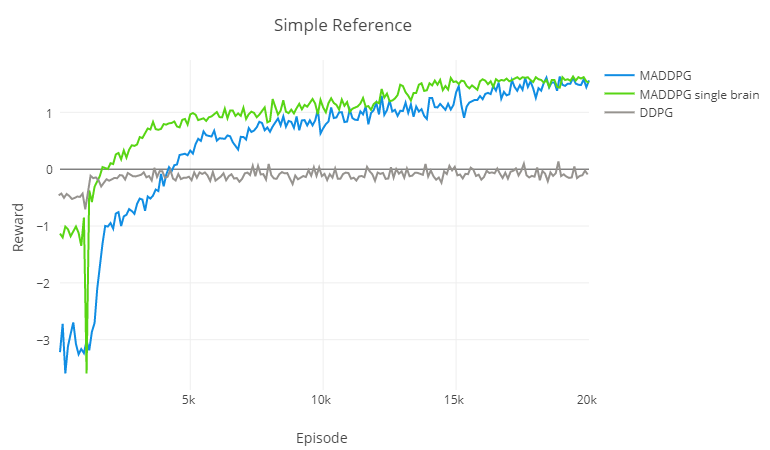
\includegraphics [scale=0.6] {my_folder/images/ch5/sr-rew.png}
	\caption{Графики согласованности взаимодействия для двух агентов в сценарии \textit{Simple Reference}. Результаты обучения по алгоритму MADDPG, MADDPG с одним мозгом и DDPG.}
	\label{fig:result-sr-rew}
\end{figure}

\begin{figure}[ht!]
	\center
	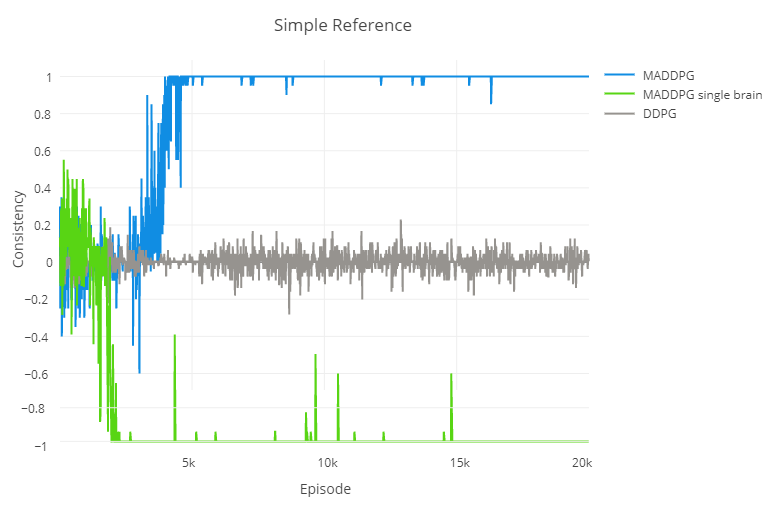
\includegraphics [scale=0.6] {my_folder/images/ch5/sr-comm.png}
	\caption{Графики согласованности взаимодействия для двух агентов в сценарии \textit{Simple Reference}. Результаты обучения по алгоритму MADDPG, MADDPG с одним мозгом и DDPG.}
	\label{fig:result-sr-comm}
\end{figure}

Мы построили график вознаграждения для двух агентов, которй представлены на \firef{fig:result-sr-rew}. На этих графиках синяя кривая - результат, обученный MADDPG, зеленая - одним мозгом, а серая - DDPG. Все они обучены за 20000 эпизодов.

Агенты, обученные с помощью DDPG, получают меньшее вознаграждение, чем агенты MADDPG и его варианты. Также из рендеринга игры видно, что агенты DDPG блуждают среди ориентиров, не зная, какой из них является правильной целью.

Графики на рисунке \firef{fig:result-sr-comm} показывают согласованность действий общения. Для MADDPG и его варианта, средний детерминант стремиться к 1 или -1. Это указывает на то, что агенты, обученные с помощью этих алгоритмов, могут общаться согласованно. Для агентов, обученных DDPG значение стремиться к 0, это иллюстрируют, что они не могут корректно сообщать цели.

В процессе выполнения многочисленных экспериментов мы наблюдали, что полная несходимость всегда сопровождается тем, что агенты, неспособны дифференцировать и сообщать правильные ориентиры друг другу. Тоже справедливо и для частичной сходимости, когда агенты могут перемещаться только к тем ориентирам, которые правильно сообщены другими агентами, см. \firef{fig:result-sr-non-convergency}. Это также показывает, что агентам для достижения целей необходимо сотрудничать как в физических, так и в коммуникационных действиях.

\begin{figure}[ht!]
	\center
	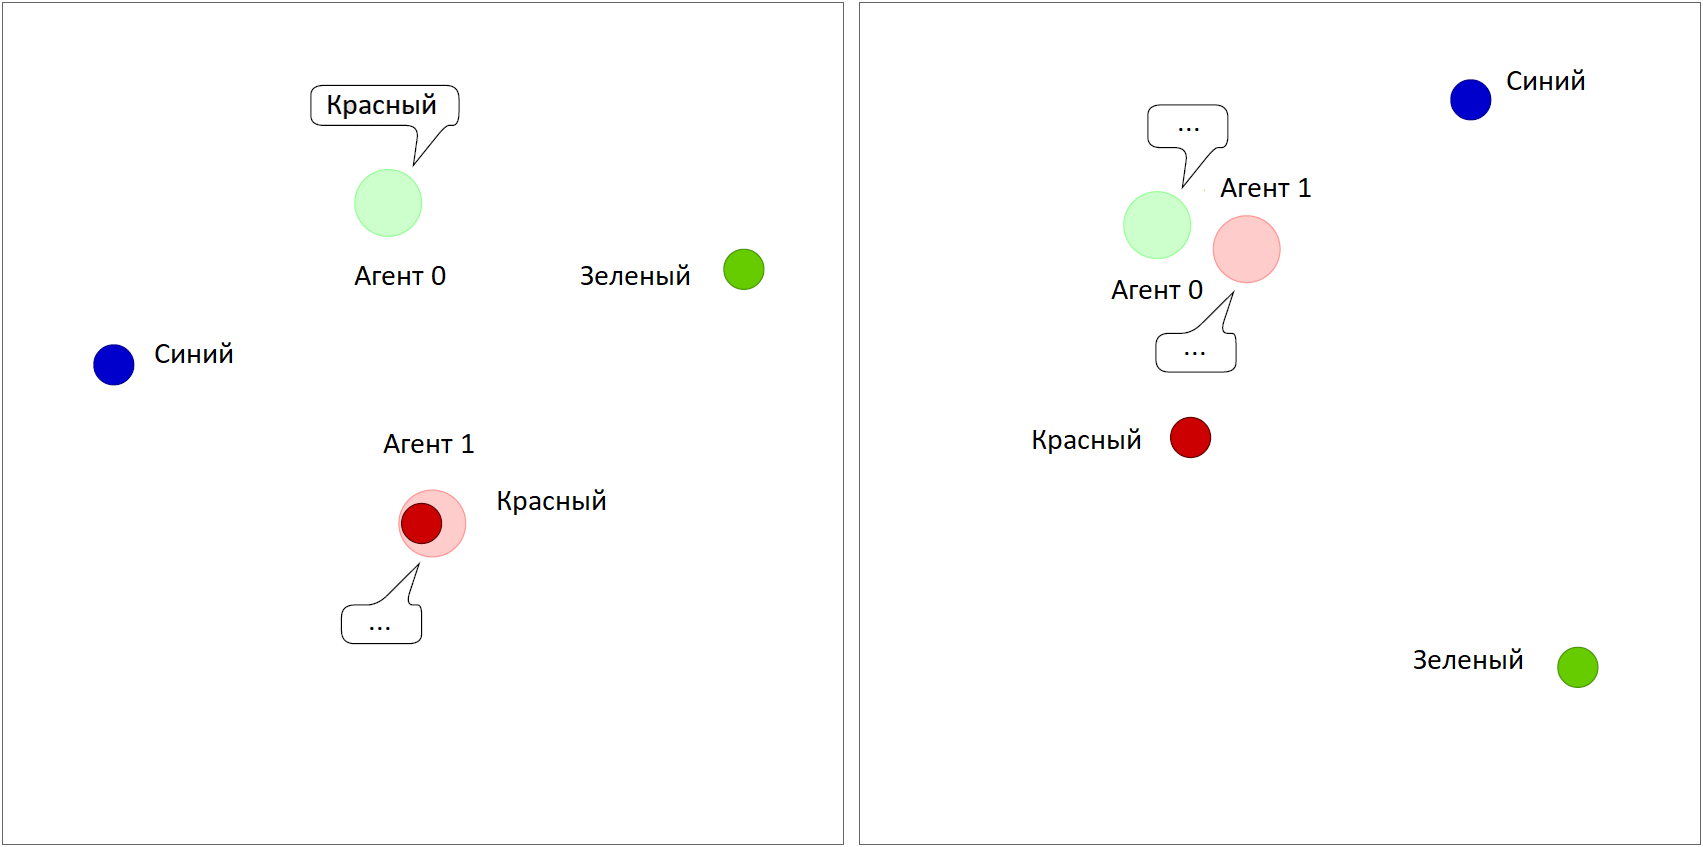
\includegraphics [scale=0.45] {my_folder/images/ch5/results-sr-non-convergency.png}
	\caption{Частичная сходимость с левой стороны: один агент перемещается к цели, а другой ждет между ориентирами. Не сходимость на правой стороне заканчивается тем, что оба агента не знают, куда двигаться и ждут между ориентирами.}
	\label{fig:result-sr-non-convergency}
\end{figure}

Наконец, между агентами возникает язык. Проведенные эксперименты показали, что при каждой тренировке агенты по-разному интерпретируют ориентиры. Например, после одной тренировки, красный ориентир может выглядеть как [1; 0; 0], а после другой, как [0; 1; 0] или [0; 0; 1].

\begin{table}[t!]
	\centering\small
	\caption{Среднее время, потраченное на обучение с различными алгоритмами в 20000 эпизодов.}
	\label{tab-sr-time}
	\begin{tabular}{|l|l|l|l|l|l|}
		\hline
		&MADDPG&MADDPG с одним мозгом\\
		\hline
		Время, 20000 эпизодов&1200с&1040с\\ \hline
	\end{tabular}
	\normalsize% возвращаем шрифт к нормальному
\end{table}

\taref{tab-sr-time} показывает время, затраченное на обучение сценарию \textit{Simple Reference} с разными алгоритмами.